% !TEX program = xelatex
% !TEX encoding = UTF-8

\documentclass[11pt, a4paper]{article} % use larger type; default would be 10pt

\usepackage{fontspec} % Font selection for XeLaTeX; see fontspec.pdf for documentation
\defaultfontfeatures{Mapping=tex-text} % to support TeX conventions like ``---''
\usepackage{xunicode} % Unicode support for LaTeX character names (accents, European chars, etc)
\usepackage{xltxtra} % Extra customizations for XeLaTeX
\usepackage{tikz}
\usetikzlibrary{arrows,calc,patterns}

\setmainfont[Ligatures=TeX]{[EBGaramond-Regular.ttf]} % set the main body font (\textrm), assumes Charis SIL is installed
%\setsansfont{Deja Vu Sans}
\setmonofont[Ligatures=TeX]{Fira Code}

% other LaTeX packages.....
\usepackage{fullpage}
\usepackage[top=2cm, bottom=4.5cm, left=2.5cm, right=2.5cm]{geometry}
\usepackage{amsmath,amsthm,amsfonts,amssymb,amscd,systeme}
\usepackage{unicode-math}
\usepackage{cancel}
\geometry{a4paper} 
%\usepackage[parfill]{parskip} % Activate to begin paragraphs with an empty line rather than an indent
\usepackage{fancyhdr}
\usepackage{listings}
\usepackage{graphicx}
\usepackage{hyperref}
\usepackage{multicol}

\renewcommand\lstlistingname{Algorithm}
\renewcommand\lstlistlistingname{Algorithms}
\def\lstlistingautorefname{Alg.}
\lstdefinestyle{mystyle}{
    % backgroundcolor=\color{backcolour},   
    % commentstyle=\color{codegreen},
    % keywordstyle=\color{magenta},
    % numberstyle=\tiny\color{codegray},
    % stringstyle=\color{codepurple},
    basicstyle=\ttfamily\footnotesize,
    breakatwhitespace=false,         
    breaklines=true,                 
    captionpos=b,                    
    keepspaces=true,                 
    numbers=left,                    
    numbersep=5pt,                  
    showspaces=false,                
    showstringspaces=false,
    showtabs=false,                  
    tabsize=2
}
\lstset{style=mystyle}

\newcommand\course{6 - Матстатистика}
\newcommand\hwnumber{Домашня КР №2}             % <-- homework number
\newcommand\idgroup{ФІ-91}                
\newcommand\idname{Михайло Корешков}  

\usepackage[framemethod=TikZ]{mdframed}
\mdfsetup{%
	backgroundcolor = black!5,
}
\mdfdefinestyle{ans}{%
    backgroundcolor = green!5,
    linecolor = green!50,
    linewidth = 1pt,
}

\pagestyle{fancyplain}
\headheight 35pt
\lhead{\idgroup \\ \idname}
\chead{\textbf{\Large \hwnumber}}
\rhead{\course \\ \today}
\lfoot{}
\cfoot{}
\rfoot{\small\thepage}
\headsep 1.5em

\linespread{1.2}

\begin{document}

\section*{№1}
\begin{mdframed}
    $$n = 15$$
    $$\xi_i \sim Exp(\lambda) - iid$$

    Побудувати $0.95$-довірчий інтервал для 
    \begin{itemize}
        \item $M\xi_1$
        \item $\sqrt{D\xi_1}$
    \end{itemize}
\end{mdframed}

\subsection*{1.}

Перш за все зазначу, що $M\xi_i = \frac{1}{\lambda}$.

Let $T_1(\vec X) = \overline X$. Це змістовна та незміщена оцінка $M\xi_1$.
Хочемо привести цю статистику до відомого розподілу.

Зауважу що $\chi^2(n) \sim Gamma(\frac{n}{2}, 2)$.

Спочатку перетворю $\xi_i$ наступним чином:\\
Нехай $\eta_i = 2\lambda\xi_i$.
$F_\eta(x) = F_\xi(\frac{x}{2\lambda})$.
$f_\eta(x) = \frac{\lambda}{2\lambda} e^{-\frac{\lambda}{2\lambda}x} = \frac{1}{2}e^{-\frac{x}{2}}$.
Тобто 
$$2\lambda\xi_i = \eta_i \sim \exp(\frac{1}{2}) \sim \chi^2(2)$$.

Тоді 
$$2 \lambda \sum_i \xi_i \sim \chi^2(2n)$$ 
- отримали табличний розподіл.

Let $\gamma = 0.95$.
$$P\left(g_1 < 2 \lambda \sum_i \xi_i < g_2\right) = \gamma$$
$$P\left(\frac{g_1}{2\sum_i \xi_i} <  \lambda  < \frac{g_2}{2\sum_i \xi_i}\right) = \gamma$$
$$P\left(\frac{2\sum_i \xi_i}{g_2} <  \frac{1}{\lambda}  < \frac{2\sum_i \xi_i}{g_1}\right) = \gamma$$

Використовую центральний інтервал із площею $\gamma$, залишаючи ліворуч та праворуч 
інтервали із площами $\frac{1-\gamma}{2}$ кожен. 
Це відповідає
$$g_1 = F^{-1}_{\chi^2(2n)}\left(\frac{1-\gamma}{2}\right)$$ 
$$g_2 = F^{-1}_{\chi^2(2n)}\left(\frac{1+\gamma}{2}\right)$$ 

Отримали $\gamma$-довірчий інтервал 
$$\left(\frac{2\sum_i \xi_i}{g_2} ; \frac{2\sum_i \xi_i}{g_1}\right)$$

Обчислимо його у Python:
\begin{figure}[h]
    \centering
    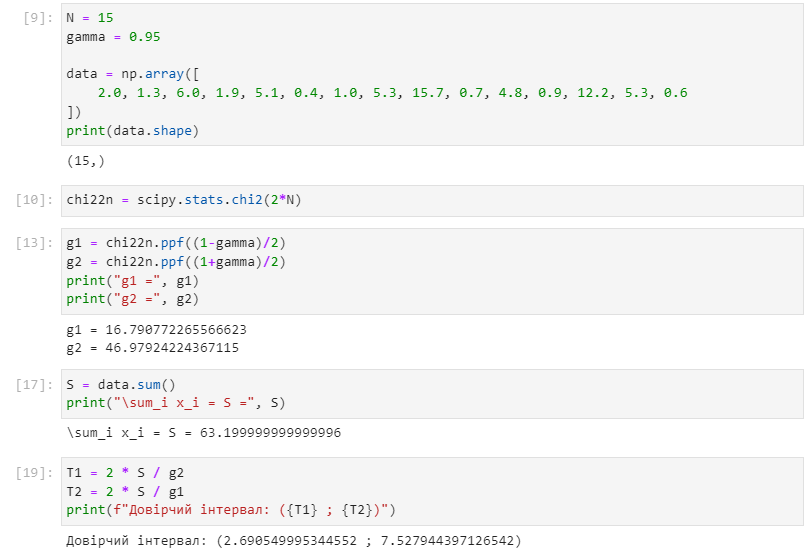
\includegraphics[width=0.9\textwidth]{img/task1.png}
\end{figure}

\begin{mdframed}[style=ans]
    Маємо $0.95$-довірчий інтервал для $M\xi_1$:
    $$P\left(2.69 < M\xi < 7.53\right) = 0.95$$
\end{mdframed}

\subsection*{2.}
Стандартне відхилення має вигляд
$$\sigma = \sqrt{D\xi_1} = \sqrt{\frac{1}{\lambda^2}} = \frac{1}{\lambda} = M\xi_1$$
Тобто підходить інтервал, знайдений в попередньому пункті
\pagebreak

\section*{№2}
\begin{mdframed}
    $$\xi_i \sim \mathcal{N}(\mu, \sigma^2) - iid;$$

    Знайти $0.95$-довірчі інтервали для $\mu$ та $\sigma$
\end{mdframed}

\subsection*{1. $\mu$}
Знаємо ОМП $\mu$:
$$T_1(\vec X) = \overline X$$

% \begin{mdframed}[backgroundcolor=blue!10]
%     $$L(\vec X, \mu, \sigma^2) = \exp\left\{ - \frac{1}{2\sigma^2}\sum_i (x_i-\mu)^2 \right\}$$
%     $$\frac{\partial}{\partial \mu} \ln L(\vec X, \mu, \sigma^2) = - \frac{1}{\sigma^2} \sum_i (x_i-\mu) = \frac{n}{\sigma^2}\left( \mu - \overline X \right) = 0$$
%     $$\implies \mu = \overline X$$
%     Дійсно ОМП
% \end{mdframed}

Знаємо ОМП $\sigma^2$:
$$T_2(\vec X) = S^2 = \frac{1}{n-1} \sum_{{i=1}}^n (X_i - \overline X)^2$$

Знаємо, що $$T = \frac{\overline{X} - \mu}{S \fracslash \sqrt{n}} \sim t(n-1)$$
- має розподіл Ст'юдента із $n-1$ степенями свободи - розподіл не залежить від $\mu$, $\sigma^2$.

Будуємо інтервал:
$$P(g_1 < T < g_2) = \gamma;$$
$$\text{let } g_1 = t_{n-1}^{-1}(\frac{1-\gamma}{2}); \; g_2 = t_{n-1}^{-1}(\frac{1+\gamma}{2})$$

З іншого боку
$$P(g_1 < T < g_2) = P(g_1 < \frac{\overline{X} - \mu}{S \fracslash \sqrt{n}} < g_2) = $$
$$= P(\frac{S}{\sqrt n} g_1 < \overline X - \mu < \frac{S}{\sqrt n}  g_2) = $$
$$= P(\overline X - \frac{S}{\sqrt n} g_2 < \mu < \overline X - \frac{S}{\sqrt n} g_1) = \gamma$$

Маємо інтервал для $\mu$.

\subsection*{2. $\sigma$}
Знаємо:
$$\zeta = \frac{n-1}{\sigma^2} S^2 \sim \chi^2(n-1)$$

Будуємо інтервал
$$P(g_1 < \zeta < g_2) = \gamma$$
$$\text{let } g_1 = F_{\chi^2(n-1)}^{-1}(\frac{1-\gamma}{2}); \; g_2 = F_{\chi^2(n-1)}^{-1}(\frac{1+\gamma}{2})$$

З іншого боку
$$P(g_1 < \frac{n-1}{\sigma^2} S^2 < g_2) = $$
$$= P(\frac{1}{g_2} < \frac{\sigma^2}{S^2(n-1)} < \frac{1}{g_1}) = $$
$$= P(\frac{S^2(n-1)}{g_2} < \sigma^2 < \frac{S^2(n-1)}{g_1}) = \gamma$$

Маємо інтервал для $\sigma^2$.

\subsection*{3. Обчислення}

\begin{figure}[h]
    \centering
    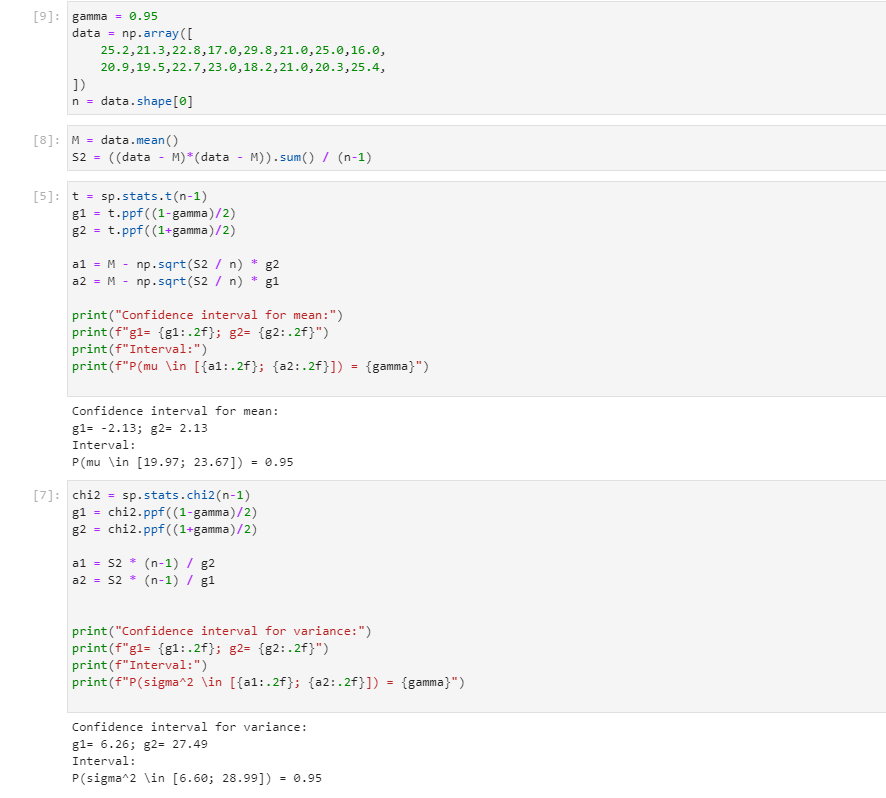
\includegraphics[width=1\textwidth]{img/task2.png}
\end{figure}

\begin{mdframed}[style=ans]
    $$P(\mu \in [19.97; 23.67]) = 0.95$$
    $$P(\sigma^2 \in [6.60; 28.99]) = 0.95$$
\end{mdframed}

\pagebreak

\section*{№3}

\begin{mdframed}
    $$X_i \sim \mathcal N (a,1)$$
    $$H0: \overline X \in [12.0; 12.6]$$
    $$H0 - \text{гіпотеза, що } \mu = 12.3$$
    $$H1: \overline X \notin [12.0; 12.6]$$
    $$H1 - \text{гіпотеза, що } \mu \ne 12.3$$
    $$n = 36$$
    $$\sigma = 1$$

    Обчислити рівень значущості критерію $\alpha$
\end{mdframed}

$$\overline X \sim \mathcal{N}(\mu, \frac{\sigma^2}{n})$$
$$\eta = \frac{\sqrt n (\overline X - \mu)}{\sigma} = 6(\overline X - 12.3) \sim \mathcal{N}(0,1)$$

$$\alpha(\mu) = P(H1 \;|\; H0)$$
$$\alpha(\mu) = P(\overline X \notin [12; 12.6] \; | \; \mu = 12.3) = $$
$$= P(\eta \notin [-0.3\cdot 6; 0.3 \cdot 6] \;|\; \mu = 12.3) = $$
$$= 1-\left(\Phi_{0,1}(1.8)-\Phi_{0,1}(-1.8)\right) = 2 - 2\Phi_{0,1}(1.8) \approx 0.0719$$

\begin{mdframed}[style=ans]
    Отже, рівень значущості має значення приблизно $0.072$
\end{mdframed}


\section*{№4}
\begin{mdframed}
    $$n = 10$$
    $$X_i \sim Exp(\lambda) - iid$$
    $$H0: \mu = 50000;\quad H1: \mu = 70000;\quad \alpha=0.05$$
\end{mdframed}

Найпотужнішим критерієм буде критерій Неймана-Пірсона, що визначається критичною областю виду 
$$\mathcal K = \left\{ \vec x :\; \frac{L_1}{L_0} \ge K \right\}$$
, де константа $K$ вибирається з умови заданої потужності:
$$P(\frac{L_1}{L_0} \ge K \;|\; H0) = \alpha$$

$$L(\vec x, \lambda) = \prod_{i=1}^n \lambda e^{-\lambda x_i} = \lambda^n e^{-\lambda n \overline X }$$

$$\frac{L_1}{L_0} = \left(\frac{\mu_0}{\mu_1}\right)^n e^{-n \overline X \left(\frac{1}{\mu_1} - \frac{1}{\mu_0}\right)} \ge K$$
$$e^{-n \overline X \left(\frac{1}{\mu_1} - \frac{1}{\mu_0}\right)} \ge K_1$$
$$+n \left(\overline X \left(\frac{1}{\mu_0} - \frac{1}{\mu_1}\right)\right) \ge K_2$$
$$\overline X \ge K_3$$
Тобто умова для вибору K має вигляд
$$P(\overline X \ge K \;|\; H0) = \alpha$$

$$\overline X \sim Gamma(n, n \lambda), \text{ як відома сума в.в.}$$
$$\eta = 2 n \lambda \overline X \sim Gamma(n, frac{1}{2}) = \chi^2(2n)$$
або інакше,
$$\eta = \frac{2n}{\mu} \overline X \sim \chi^2(2n)$$

$$P(\overline X \ge K \;|\; H0) = P(\eta \ge \frac{2n}{\mu_0} K) = 1 - P(\eta \le \frac{2n}{\mu_0} K) = \alpha$$
$$\frac{2n}{\mu_0} K = F_{\chi^2(2n)}^{-1}(1-\alpha) = 31.4$$
$$K = 78526$$

\begin{mdframed}[style=ans]
    Тобто маємо статичтичний критерій для відидання гіпотези H0:
    $$\overline X \ge 78526$$
\end{mdframed}


\section*{№5}

















\end{document}

